\documentclass[11pt]{article}

\usepackage[margin=1in]{geometry}
\usepackage{amsmath,amssymb,amsthm}
\usepackage{graphicx}
\usepackage{hyperref}

\newtheorem{theorem}{Theorem}
\newtheorem{lemma}{Lemma}
\newtheorem{remark}{Remark}

\newcommand{\R}{\mathbb{R}}
\newcommand{\E}{\mathcal{E}}
\newcommand{\I}{\mathcal{I}}
\newcommand{\Lag}{\operatorname{Lag}}
\newcommand{\spanop}{\operatorname{span}}
\newcommand{\supp}{\operatorname{supp}}
\newcommand{\eps}{\varepsilon}

\title{Positive Definiteness of the Semidiscrete Moment-Measure Newton Matrix}
\author{agent\_lane\_05}
\date{July 18, 2026}

\begin{document}
\maketitle

\section*{Status}

This is a partial result for Bonnet--Rubinstein, \emph{Quantitative Stability and Numerical Resolution of the Moment Measure Problem}, arXiv:2604.09914~\cite{BR}.  The source paper leaves two questions for future work in Section~4.3: invertibility of the regularized Newton matrix used in Algorithm~4.1, and convergence of the damped Newton method.  The result below proves the invertibility part at every full-cell iterate $\Phi\in U$.  It does not prove global convergence, nor does it address how far the iterates remain from the boundary of $U$.

\section*{Source Passage}

The source defines the regularized matrix on page~22:

\begin{center}
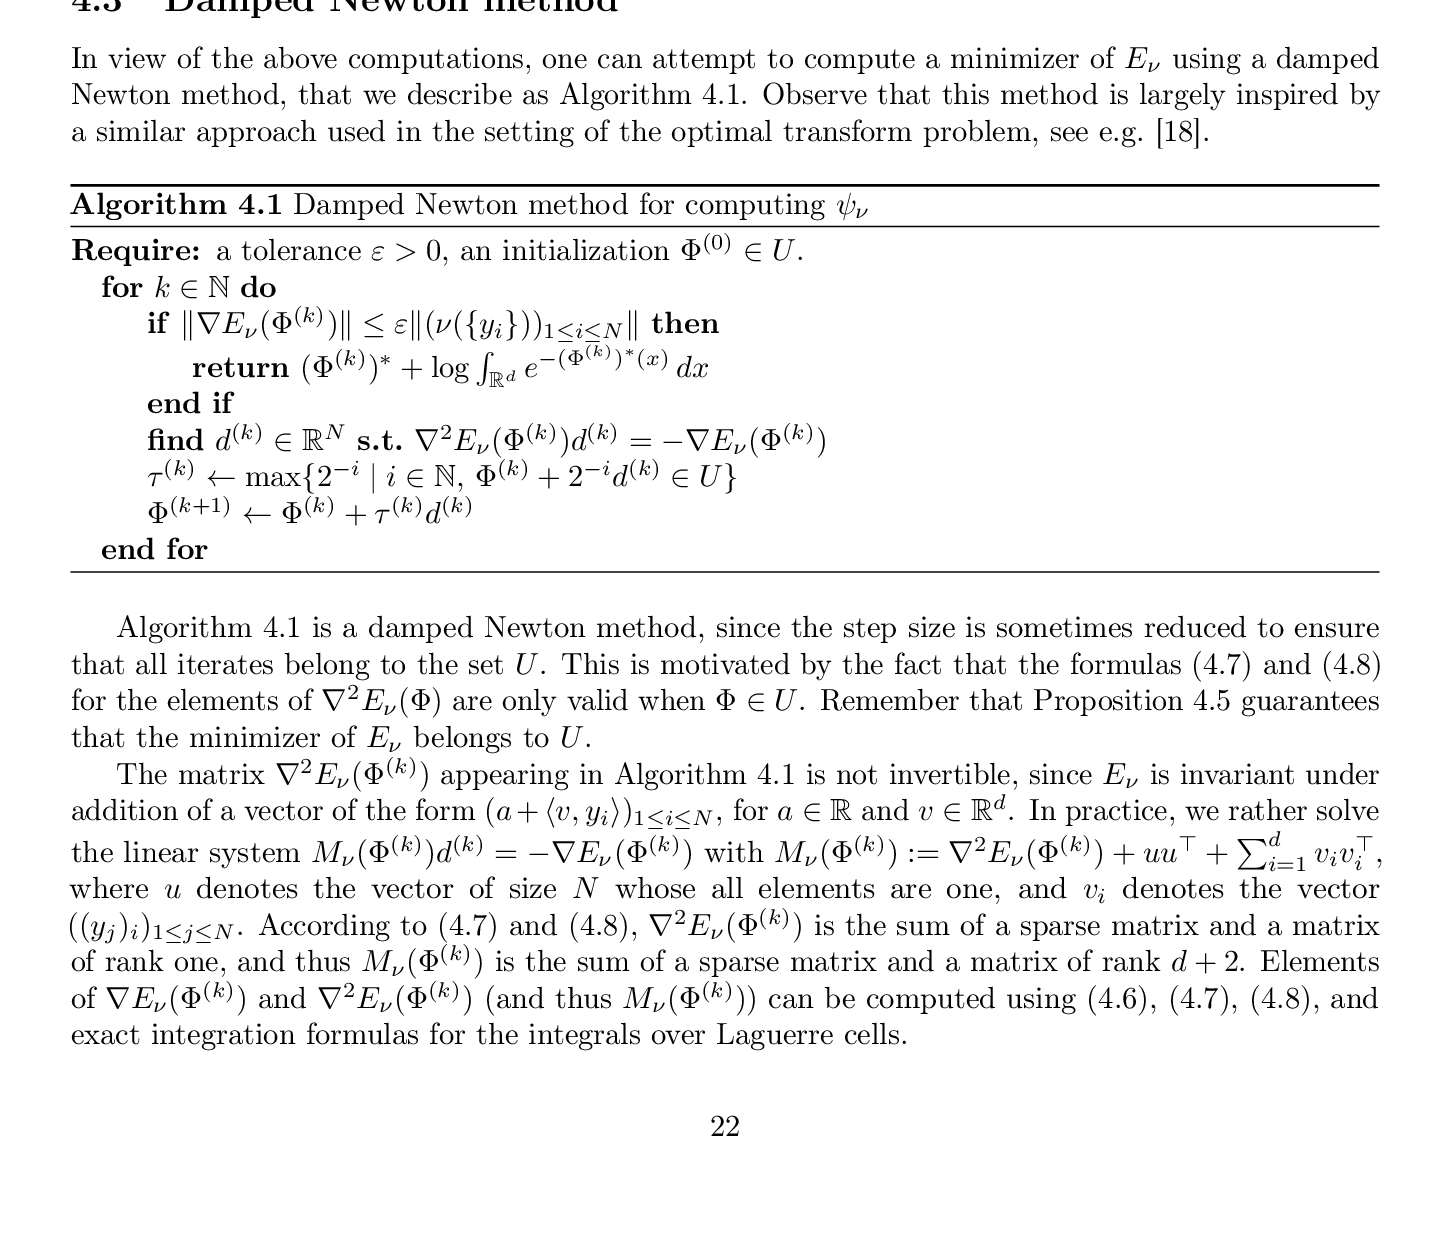
\includegraphics[width=0.95\linewidth]{figures/open_problem_crop_page22_matrix_definition.png}
\end{center}

The explicit future-work sentence appears at the top of page~23:

\begin{center}
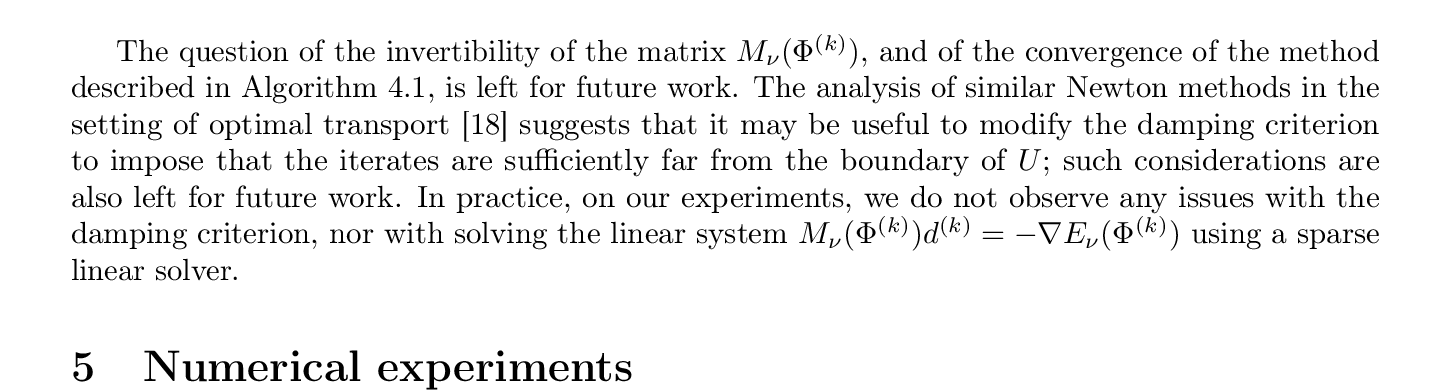
\includegraphics[width=0.95\linewidth]{figures/open_problem_crop_page23_future_work.png}
\end{center}

\section*{Transcription of the Target}

In Section~4.3, after defining
\[
M_\nu(\Phi)=\nabla^2E_\nu(\Phi)+u u^\top+\sum_{\alpha=1}^d v_\alpha v_\alpha^\top,
\]
where $u=(1,\ldots,1)$ and $v_\alpha=((y_j)_\alpha)_{1\le j\le N}$, Bonnet--Rubinstein write:
\begin{quote}
The question of the invertibility of the matrix $M_\nu(\Phi^{(k)})$, and of the convergence of the method described in Algorithm 4.1, is left for future work.
\end{quote}

\section*{Definitions}

Let $\nu=\sum_{i=1}^N p_i\delta_{y_i}$ be a finitely supported probability measure on $\R^d$, with all $p_i>0$, centered, and not supported on a hyperplane.  Thus the vectors
\[
u=(1,\ldots,1),\qquad v_\alpha=((y_i)_\alpha)_{i=1}^N,\quad 1\le \alpha\le d,
\]
are linearly independent in $\R^N$.  For $\Phi\in\R^N$, put
\[
\Phi^*(x)=\max_{1\le i\le N}(\langle x,y_i\rangle-\Phi_i)
\]
and
\[
E_\nu(\Phi)=\sum_i p_i\Phi_i-\log\int_{\R^d}e^{-\Phi^*(x)}\,dx.
\]
Let $U$ be the open set of $\Phi$ for which every Laguerre cell
\[
\Lag_i(\Phi)=\{x:\langle x,y_j-y_i\rangle\le \Phi_j-\Phi_i\text{ for all }j\}
\]
has nonempty interior.  The source paper computes $\nabla^2E_\nu(\Phi)$ for $\Phi\in U$.

\section*{Proof Intuition}

The Hessian of $E_\nu$ cannot be invertible, because adding $a+\langle b,y_i\rangle$ to the entries $\Phi_i$ only translates and rescales the density $e^{-\Phi^*}$; this gives exactly the $(d+1)$ affine null directions.  The source regularization adds rank-one terms in precisely those directions.  The only possible obstruction would be an extra hidden null direction of the Hessian.  The key point is that such a direction would make the normalized densities associated to $\Phi+t h$ and $\Phi-t h$ agree up to translation to first order.  Looking inside the interiors of the Laguerre cells forces $h_i$ to be affine in $y_i$, so no hidden null direction exists.

\section*{Theorem}

\begin{theorem}
\label{thm:pd}
Under the hypotheses above, for every $\Phi\in U$ the matrix
\[
M_\nu(\Phi)=\nabla^2E_\nu(\Phi)+u u^\top+\sum_{\alpha=1}^d v_\alpha v_\alpha^\top
\]
is symmetric positive definite.  In particular, the linear system with coefficient matrix $M_\nu(\Phi^{(k)})$ in Algorithm~4.1 of~\cite{BR} has a unique solution at every iterate $\Phi^{(k)}\in U$.
\end{theorem}

\section*{Proof}

Let
\[
A=\{(a+\langle b,y_i\rangle)_{i=1}^N:a\in\R,\ b\in\R^d\}\subset\R^N
\]
be the affine-value subspace.  Since the support of $\nu$ is not contained in a hyperplane, $\dim A=d+1$, and $A=\spanop\{u,v_1,\ldots,v_d\}$.

We first record the kernel statement needed below.

\begin{lemma}
\label{lem:kernel}
For every $\Phi\in U$, the Hessian $H(\Phi):=\nabla^2E_\nu(\Phi)$ is positive semidefinite and
\[
\ker H(\Phi)=A.
\]
\end{lemma}

\begin{proof}
The linear part $\sum_i p_i\Phi_i$ has no second derivative, so $H(\Phi)$ is the Hessian of
\[
I(\Phi)=-\log\int_{\R^d}e^{-\Phi^*(x)}\,dx.
\]
The Prekopa--Leindler argument used in Proposition~3.3 of~\cite{BR} gives convexity of this functional on the finite-dimensional family of lower convex envelopes determined by the values $\Phi_i$.  Hence $H(\Phi)$ is positive semidefinite.

For $h\in A$, say $h_i=a+\langle b,y_i\rangle$, one has
\[
(\Phi+t h)^*(x)=\Phi^*(x-tb)-ta.
\]
Thus $I(\Phi+t h)$ is affine in $t$, and therefore $h\in\ker H(\Phi)$.  So $A\subseteq\ker H(\Phi)$.

It remains to rule out further null directions.  Fix $h\in\R^N$ and, for small $t$, set
\[
\psi_t=(\Phi+t h)^*,\qquad
Z_t=\int_{\R^d}e^{-\psi_t(x)}\,dx,\qquad
\rho_t=Z_t^{-1}e^{-\psi_t}.
\]
Because $\Phi\in U$, all cells have interior points with strict inequalities; after decreasing $|t|$ if necessary, each support point remains active.  Let $\varphi_t=(\Phi+t h)^{**}$ be the lower convex envelope of the values $\Phi_i+t h_i$ on $\{y_i\}$.

Consider the symmetric second difference
\[
D(t)=\frac{E_\nu(\Phi+t h)+E_\nu(\Phi-t h)}2-E_\nu(\Phi).
\]
The linear part of $E_\nu$ cancels.  Moreover, the convex function $(\varphi_t+\varphi_{-t})/2$ is bounded above by $\varphi_0$ because it takes values at most $\Phi_i$ at all $y_i$; therefore
\[
\left(\frac{\varphi_t+\varphi_{-t}}2\right)^*\ge \varphi_0^*,
\qquad
\I\!\left(\frac{\varphi_t+\varphi_{-t}}2\right)\ge \I(\varphi_0).
\]
Applying the quantitative midpoint convexity estimate of~\cite[Proposition~3.3]{BR} to $\varphi_t$ and $\varphi_{-t}$ gives, for some translation $z_t\in\R^d$,
\[
D(t)\ge c_{\Phi,h,d}\,
\|\rho_t-\rho_{-t}(\,\cdot-z_t)\|_{L^1(\R^d)}^2
\]
for all sufficiently small $|t|$; the value of the positive constant is immaterial.

Suppose now that $h^\top H(\Phi)h=0$.  Then $D(t)=o(t^2)$.  Hence, along a sequence $t_n\to0$, there are translations $z_n$ with
\[
\|\rho_{t_n}-\rho_{-t_n}(\,\cdot-z_n)\|_{L^1}=o(|t_n|).
\]
The density $\rho_0$ is not translation-invariant in any nonzero direction.  More quantitatively, since $\rho_0$ is a polyhedral log-concave density with finite weighted facet perimeter, the map $r\mapsto \rho_0(\cdot-r\theta)$ has a nonzero $L^1$ first variation for every $\theta\in S^{d-1}$; compactness of $S^{d-1}$ gives $c>0$ such that
\[
\|\rho_0-\rho_0(\,\cdot-r\theta)\|_{L^1}\ge c r+o(r)
\]
uniformly in $\theta$.  Since $\rho_{\pm t}=\rho_0+O(t)$ in $L^1$, the preceding $o(|t_n|)$ estimate forces $z_n=O(t_n)$.  Pass to a subsequence with $z_n/t_n\to w$.

Let $C_i$ be a compact subset of the interior of $\Lag_i(\Phi)$ with positive Lebesgue measure.  On $C_i$, for $n$ large, the active index in the maximum defining $\psi_{\pm t_n}$ is still $i$, and also $x-z_n\in\Lag_i(\Phi)$ after shrinking $C_i$ slightly.  Writing
\[
\bar h=\sum_i q_i h_i,\qquad
q_i=\int_{\Lag_i(\Phi)}\rho_0(x)\,dx,
\]
we have the first-order expansions on $C_i$:
\[
\rho_{t_n}(x)=\rho_0(x)\left(1+t_n(h_i-\bar h)+o(t_n)\right),
\]
and
\[
\rho_{-t_n}(x-z_n)
=\rho_0(x)\left(1+\langle z_n,y_i\rangle-t_n h_i+t_n\bar h+o(t_n)\right).
\]
The $L^1$ difference being $o(|t_n|)$ forces the coefficient of $t_n$ in the difference to vanish on every cell:
\[
2(h_i-\bar h)-\langle w,y_i\rangle=0,\qquad 1\le i\le N.
\]
Thus $h_i=\bar h+\langle w/2,y_i\rangle$, so $h\in A$.  This proves $\ker H(\Phi)\subseteq A$, and the lemma follows.
\end{proof}

We now finish the proof of the theorem.  For any $h\in\R^N$,
\[
h^\top M_\nu(\Phi)h
=h^\top H(\Phi)h+(h\cdot u)^2+\sum_{\alpha=1}^d(h\cdot v_\alpha)^2.
\]
By Lemma~\ref{lem:kernel}, the first term is nonnegative.  If the displayed expression is zero, then $h\in\ker H(\Phi)=A$, while also $h$ is orthogonal to every vector spanning $A$.  Hence $h\in A\cap A^\perp=\{0\}$.  Therefore $M_\nu(\Phi)$ is positive definite.

\section*{Verification Notes}

The proof is analytic.  A small independent script, \texttt{code/check\_d1\_newton\_matrix.py}, checks the one-dimensional explicit Hessian formula for random full-cell configurations.  Run from the repository root:
\begin{verbatim}
conda run --no-capture-output -n sandbox python \
  runs/fa_banach_001/solutions/partial/2604.09914_newton_matrix_invertibility/\
  code/check_d1_newton_matrix.py
\end{verbatim}
On July 18, 2026, it sampled 1500 configurations, found no failures, and reported minimum regularized eigenvalue approximately $0.12924$.  This numerical check is not used in the proof.

\section*{Limitations and Novelty Check}

This packet proves only the invertibility of $M_\nu(\Phi)$ for $\Phi\in U$.  It does not prove convergence of Algorithm~4.1, does not give lower bounds uniform near the boundary of $U$, and does not justify any adaptive damping rule.  The target is finite-dimensional convex/numerical analysis rather than a core Banach-space structure problem; it was nevertheless retained because the extracted question is precise and the proof is packet-sized.

The bounded local novelty check searched the run registry, solution index, attempts, proof gaps, and ledger for arXiv:2604.09914 and the terms ``moment measure'', ``Newton matrix'', ``damped Newton'', and ``Laguerre''.  No duplicate packet for this question was found.  No broad external web or MathSciNet-style literature search was performed, so novelty confidence is local-to-run rather than global.

\section*{Human Review Recommendation}

Review the first-order rigidity step in Lemma~\ref{lem:kernel}: specifically, the passage from $L^1$ closeness of $\rho_t$ and a translated $\rho_{-t}$ at order $o(t)$ to the affine formula $h_i=\bar h+\langle w/2,y_i\rangle$.  This is the only delicate point; the final positive-definiteness argument is then immediate.

\begin{thebibliography}{9}
\bibitem{BR}
G. Bonnet and Y. A. Rubinstein,
\emph{Quantitative Stability and Numerical Resolution of the Moment Measure Problem},
arXiv:2604.09914, 2026.
\end{thebibliography}

\end{document}
